\chapter{Method}

This section presents the data used for training and evaluating models, which models that are to be tested and how the text will is processed to be of appropriate format for the models. 

The financial indices which are considered in this project is the S\&P 500 and the US treasury rate with 1 and 3 years to maturity. S\&P 500 (\textit{Standard \& Poor's}) is a stock market index reflecting the performance of the 500 largest companies listed on the stock exchanges in the United States.

The US Treasury rate with maturity $n$ is the yield on a government zero coupon bond with the same maturity. 

\section{Data Collection and Pre-Processing}

All models are trained on two datasets - a labeled movie review dataset from IMDb for benchmarking, and an unlabeled financial news dataset from Reuters for the financial interpretation. 

\subsection{IMDd Dataset - Benchmarking}

The IMDb dataset is a commonly used benchmarking dataset for binary classification of text data. The dataset was compiled by \citet{maas-EtAl:2011:ACL-HLT2011} and contains 50,000 polarized movie reviews with 25,000 positive and negative reviews respectively. Evaluating models on this dataset can validate that the models can capture some meaningful information from text data and thus give better insight about the performance on the financial task. 

\subsection{Reuters Financial News Dataset}

The corpus used for this project consists of 109,110 financial news articles from Reuters. It was first compiled and used by \citet{ding2014using} for predicting stock price direction. Only the titles of the news data is used to train the model, as suggested by \citet{ding2014using}. The reasoning behind this is that including the contents of the articles does not significantly improve the model. 

The data contains financial news regarding the US market from the 10th of October 2006 to the 11th of November 2013, with approximately 5 - 50 news articles per day and is \textcolor{red}{publicly available. How do i cite this? Links under appendix or references? \url{https://github.com/duynht/financial-news-dataset}}

\subsubsection*{Pre-Processing}

The first part of the pre-processing of text data is rather similar regardless of what the intended model to use is. The intersection of dates available with news data and financial data is assessed and headlines for these days are extracted. The text is quite clean since it is the headlines of published news articles, so it does not require as much cleaning as for instance a corpus of tweets. 

The next step of the pre-processing is to tokenize the data. This is done differently depending on what model to use, but a parameter that is set for all models is the \textit{vocabulary size}. The vocabulary size is simply the amount of words to keep track of. Keras has a tokenization functionality which includes words based on frequency - the most common words are included. How the tokenization is performed for each model is explained more carefully under \textcolor{red}{each section. MAKE SURE THESE SECTIONS ARE REASONABLE} 

For some of the used models the natural language processing part can be seen as pre-processing, for instance when pre-trained word embeddings are used. This is explained further under each model.

\section{Text Vectorization}
Some text vectorization techniques are jointly trained with the classification model, and thus not possible to isolate from the model. Others can be trained both jointly and used as a pre-processing layer for another model. This project uses three vectorization techniques. In all of the techniques except for Sentence-BERT, the news titles for one day is concatenated to one document representing the news of that day. 

The news dataset contains 27,617 unique words when converted to lower case. 

\subsection{TF-IDF}

Term Frequency - Inverse Document Frequency (TF-IDF) is purely a pre-processing technique which outputs large dimensional vectors of the same length as the vocabulary size. This can then be fed into any model. As stated in the previous chapter the order of words is not preserved in this technique, which does not make it suitable to use as input to a recurrent network. 

\subsection{GloVe}

For the word embeddings, pre-trained word vectors using the GloVe-model is used. The vectors have been trained on a dump of Wikipedia from 2014 containing 1.6 billion tokens and the English Gigaword fifth edition dataset, containing 4.3 billion tokens \citep{pennington2014glove}. 400,000 uncased words with an embedding size of 300 dimensions are represented in the used GloVe dictionary. Of the 22,415 words in the news data, 22,107 were available as pre-trained GloVe embeddings. 

The tokenization for the GloVe-models first converted all words to lower case and reformed some words such as "won't" and "can't" to "will not" and "can not". This allows for more words to be initialized with pre-trained embeddings since contracted words are handled differently by different tokenizers. The tokenization is done using the tokenizer from Keras.  

For non-sequential models, the data is converted from $w \times d$ dimensions to $1 \times d$, where $w$ is the number of words in the concatenated news titles for one day and $d$ is the embedding dimensions, here 300. This is done by taking the element-wise average over all $d$ dimensions. In the models using the embeddings as non-trainable pre-processing, this is simply done before the data is fed into the model. In the models where the training of the embeddings are continued, a custom layer in Keras computes the element-wise average after the embedding layer, where the data has been inputted as token indices and the pre-trained embeddings are set in the embedding layer.

For sequential models, the order of words in the titles is kept intact. The number of words in the news titles for one day is shown in Figure~\ref{fig:num_words}. In order for each text sample to have the same size, a maximum sentence length is set. Longer sequences are cut of, shorter sequences are padded with zeros. The maximum sentence length is set to 800 for the news data, which well covers the majority of the samples. 

\begin{figure}[h]
\centering
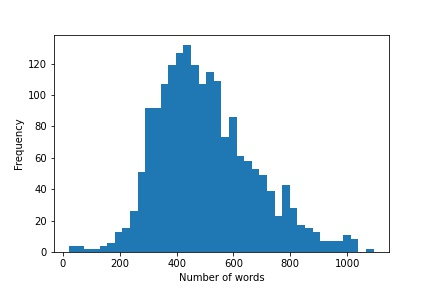
\includegraphics[width=0.8\textwidth]{Figures/wordcount.jpg}
\caption{Histogram of the number of words in the concatenated news titles for one day. }
\label{fig:num_words}
\end{figure}

\subsection{BERT}





\section{Models}

\subsubsection*{Random Classifier}

For an imbalanced rather small dataset, a random classifier can provide a basic understanding of what performance to beat to ensure some predictive power in a model. The random classifier is trained on the training set to respect the ratios of class labels, and then randomly predicts with the same distribution of classes on the validation/test data. 

The random classifier used in this project only relies on the target variables, so it is not interesting to classify it as sequential or not.  

\subsection{Non-sequential Input Models}

These models are only used with non-sequential data as input, i.e. TF-IDF, average GloVe-embeddings and Sentence-BERT. These vectorizations typically have dimensions 5,000 - 20,000 (TF-IDF), 300 (GloVe) and 768 (Sentence-BERT). 

\textcolor{red}{Hur väl måste dessa modeller motiveras?}

\subsubsection*{Logistic Regression}

Logistic regression is used both as a traditional benchmark and a more novel model in combination with GloVe and BERT embeddings. The logistic regression model from the python library scikit-learn is used for the implementation.

\subsubsection*{Support Vector Machine}

A support vector machine (SVM) is used with similar motivation as for the logistic regression - it serves as a well known benchmark model and is rather simple to implement and optimize.  A support vector machine for binary classification from the scikit-learn library is used. 

\subsubsection*{Feed-forward Network}

A densely connected feed-forward network is evaluated with varying number of hidden layers, nodes and dropout rate. The loss function is binary cross entropy, defined as $L(y,\hat{y}) = -\frac{1}{N} \sum_{i=1}^N y_i \log{(p(\hat{y}_i))} + (1 - y_i) \log{(1 - p(\hat{y}_i))}$. \textcolor{red}{Should have this under theoretical background} The model is trained using optimization algorithms RMSprop and Adam, evaluated by cross validation as shown in \textcolor{red}{appendix X}.



The feed-forward network is implemented using the Keras-library. 


\subsubsection*{Random Forest / XGBoost / LDA}
\textcolor{red}{Finns det någon vettig vits med att ha med dessa? Typ samma syfte \& resultat som logreg/svm, och har fokuserat främst på neuronnätverk. }


\subsection{Sequential Input Models}

These sequential models all allow further training of embedding parameters, since the first input layer is either a regular embedding layer or a BERT-embedding layer. The input dimensions are $w \times d$, where $w$ is the maximum sequence length and $d$ is the dimension of the embedding. 

\subsubsection*{Feed-forward Network}

The feed-forward network which takes sequential inputs has an embedded layer as the first layer. The weights in this layers are set to the pre-trained GloVe embeddings, and are then jointly trained continuously with the other parameters in the model. A maximum sequence length is specified and an average is taken element-wise over all the 300 embedding dimensions. The average is taken where the sum of the absolute value of the embedding vector is non-zero, i.e. the position in the sequence vector actually contains a word.

\begin{figure}[H]
    \centering
    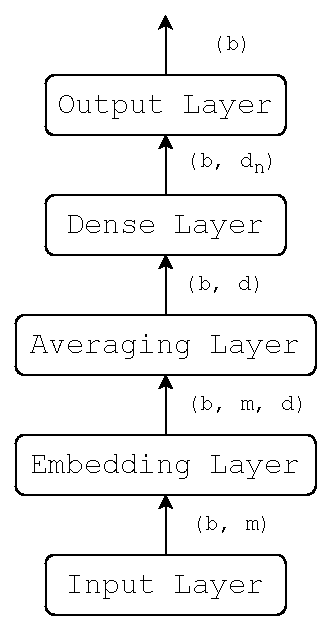
\includegraphics[width=0.3\textwidth]{Figures/figs-ff_emb.pdf}
    \caption{Schematic overview of the used feed-forward network with embedded inputs. $b$ is the batch size, $m$ is the maximum sequence length, $d$ is the embedding dimension and $d_n$ is the number of nodes in the dense layer.}
\label{fig:emb_ff}
\end{figure}

This tensor is then passed into a regular feed-forward network with rectified linear unit activation function and dropout regularization, and finally to an output layer with a sigmoid activation function. The general structure is seen in Figure~\ref{fig:emb_ff}. 

\subsubsection*{Bidirectional LSTM}

The bidirectional LSTM has the same input structure as the feed-forward network, but rather than an averaging layer over all dimensions, an LSTM layer is applied. This preserves the sequential structure of the inputs and enables the model to take the order of words into account. 

The LSTM layer is wrapped in a bidirectional layer, which 

\begin{figure}[H]
    \centering
    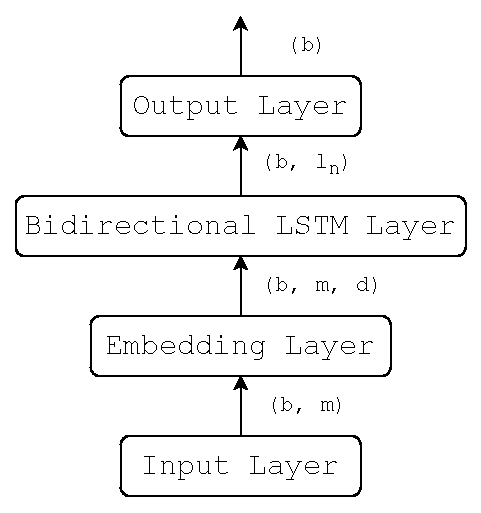
\includegraphics[width=0.4\textwidth]{Figures/figs-bidir-lstm.pdf}
    \caption{Schematic overview of a bidirectional LSTM network with sequential input data. $b$ is the batch size, $m$ is the maximum sequence length, $d$ is the embedding dimension and $l_n$ is the number of nodes in the LSTM-layer.}
\end{figure}

\subsubsection*{BERT + LSTM}



\begin{figure}[H]
    \centering
    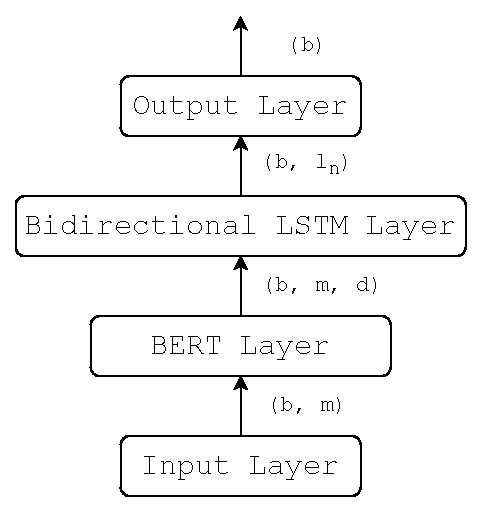
\includegraphics[width=0.4\textwidth]{Figures/figs-bert-lstm.pdf}
    \caption{Schematic overview of the used bidirectional LSTM network with sequential input data. $b$ is the batch size, $m$ is the maximum sequence length, $d$ is the BERT embedding dimension and $l_n$ is the number of nodes in the LSTM-layer.}
\end{figure}


\section{Other evaluated models}
\subsection{Hyperparameter Optimization and Prevention of Overfitting}

The selection of hyperparameters was carried out using a grid search over a selected range of parameters, where each set of parameters was evaluated using a cross validation. The number of folds was determined by the computational feasibility of the optimization. Specifically, the grid search function in the python-package sklearn was used. The tested ranges and concluded sets of parameters for all models are listed in \textcolor{red}{appendix X.}